\title{Introdução às Tabelas de Dispersão}
\date{\today}
\frame{\titlepage}

% Slide 1: Introdução às Tabelas de Dispersão
% Slide de Introdução às Tabelas de Dispersão
% Definição e Propósito: A definição e o propósito estão bem explicados. Considerar adicionar um exemplo simples de aplicação para ilustrar melhor a utilidade das tabelas de dispersão.
% Importância: O texto está claro, mas poderia ser enriquecido com exemplos específicos de como as tabelas de dispersão contribuem para o desempenho de sistemas em cenários reais.
\begin{frame}[fragile]
  \frametitle{Introdução às Tabelas de Dispersão}
  \begin{itemize}
    \item Definição e propósito das tabelas de dispersão:
      \begin{itemize}
        \item \textbf{Definição:} As tabelas de dispersão são estruturas de dados que mapeiam chaves para valores, permitindo uma recuperação eficiente dos valores associados às chaves.
        \item \textbf{Propósito:} Elas são amplamente utilizadas em diversos campos da ciência da computação e da engenharia de software devido à sua capacidade de armazenar e recuperar dados de forma rápida e eficiente.
      \end{itemize}
  \end{itemize}
\end{frame}

\begin{frame}[fragile]
  \frametitle{Introdução às Tabelas de Dispersão}
  \begin{itemize}
    
    \item Importância no armazenamento e recuperação eficiente de dados:
      \begin{itemize}
        \item Em muitas aplicações, especialmente aquelas que envolvem grandes volumes de dados, como bancos de dados, sistemas de cache e dicionários, as tabelas de dispersão são essenciais para garantir um acesso rápido e eficiente aos dados.
        \item Elas são usadas para resolver problemas como pesquisa, indexação e associação de chaves a valores, proporcionando uma maneira eficiente de armazenar e recuperar informações.
      \end{itemize}
  \end{itemize}
\end{frame}

% Slide 2: Como Funcionam as Tabelas de Dispersão
% Slide de Como Funcionam as Tabelas de Dispersão
% Processo de Mapeamento: Considerar a inclusão de um diagrama para ilustrar o processo de conversão de chaves em índices de tabela.
% Funções Hash: O texto está claro, mas adicionar um exemplo concreto de uma função hash pode ajudar a ilustrar o conceito.
\begin{frame}[fragile]
  \frametitle{Como Funcionam as Tabelas de Dispersão}
  \begin{itemize}
    \item \textbf{Processo de mapeamento de chaves para índices de tabela:}
      \begin{itemize}
        \item Utilizam funções hash para converter chaves em índices de tabela, onde os valores associados são armazenados.
        \item O objetivo é distribuir as chaves uniformemente pela tabela, minimizando colisões e facilitando uma recuperação eficiente.
        \item \textbf{Diagrama:} [Incluir um diagrama aqui que ilustre uma chave sendo convertida em um índice de tabela através de uma função hash, destacando a distribuição uniforme das chaves.]
      \end{itemize}
    
  \end{itemize}
\end{frame}
\begin{frame}[fragile]
  \frametitle{Como Funcionam as Tabelas de Dispersão}
  \begin{figure}
    \centering
    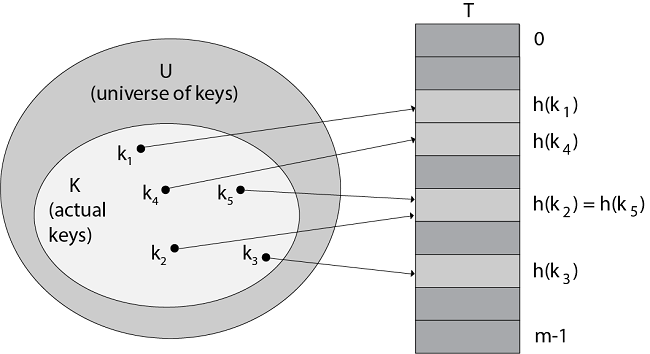
\includegraphics[width=0.8\textwidth]{aulas/aula2-hash-fig1.png}
    \caption{Caption of the Image}
  \end{figure}
\end{frame}
\begin{frame}[fragile]
  \frametitle{Como Funcionam as Tabelas de Dispersão}
  \begin{itemize}
    \item \textbf{Uso de funções hash para conversão de chaves:}
      \begin{itemize}
        \item Essenciais para a eficiência das tabelas de dispersão, as funções hash transformam chaves em índices de tabela de maneira rápida.
        \item Distribuem as chaves uniformemente, evitando colisões excessivas e otimizando o desempenho.
        \item \textbf{Exemplo Concreto:} Suponha uma função hash simples onde a chave é um número inteiro e o tamanho da tabela é 10. A função hash pode ser \(hash(k) = k \mod 10\), onde \(k\) é a chave. Se \(k = 23\), então \(hash(23) = 3\), indicando que o valor associado à chave 23 será armazenado no índice 3 da tabela.
      \end{itemize}
  \end{itemize}
\end{frame}


% Slide 3: Funções Hash
% Slide de Funções Hash
% Definição e Propriedades: A explicação está adequada. Seria útil incluir exemplos visuais para demonstrar a uniformidade e a eficiência.
% Exemplos de Funções Hash: Está bom, mas considerar adicionar exemplos de código ou pseudocódigo para as funções de hash mencionadas.
\begin{frame}[fragile]
  \frametitle{Definição e Propriedades das Funções Hash}
  \begin{itemize}
    \item \textbf{Definição:} 
      \begin{itemize}
        \item Uma função hash converte dados de tamanho variável em valores de 
        tamanho fixo, ideal para índices de tabela.
      \end{itemize}
    \item \textbf{Propriedades desejáveis:}
      \begin{itemize}
        \item \textbf{Uniformidade:} Distribui chaves de forma uniforme, 
        evitando sobrecarga em partes específicas da tabela.
        \item \textbf{Eficiência:} Rápida no cálculo, garantindo acesso ágil 
        aos dados.
        \item \textbf{Baixa probabilidade de colisão:} Minimiza casos onde 
        chaves distintas resultam no mesmo índice.
      \end{itemize}
    \item \textbf{Visualização:} Incluir um gráfico demonstrando a distribuição 
    uniforme das chaves pela tabela pode ajudar a ilustrar a uniformidade. 
    (Considerar adicionar um gráfico ou diagrama que ilustre esta propriedade.)
  \end{itemize}
\end{frame}

\begin{frame}[fragile]
  \frametitle{Exemplos de Funções Hash com Pseudocódigo}
  \begin{itemize}
    \item \textbf{Exemplos de funções hash simples com pseudocódigo:}
      \begin{itemize}
        \item \textbf{Função de Módulo:}
        \begin{mysmallverbatim}
            funcao_hash_modulo(chave, tamanho_da_tabela):
              return chave % tamanho_da_tabela
        \end{mysmallverbatim}
        \item \textbf{Função de Multiplicação:}
          \begin{mysmallverbatim}
            funcao_hash_multiplicacao(chave, tamanho_da_tabela):
              A = 0.6180339887 # constante (número de ouro - 1)
              return floor(tamanho_da_tabela * (chave * A \% 1))
          \end{mysmallverbatim}
      \end{itemize}
    \item Estes pseudocódigos ilustram métodos comuns para transformar chaves 
    em índices de tabela. A função de módulo é simples e direta, enquanto a 
    função de multiplicação utiliza uma constante para ajudar a distribuir as 
    chaves de maneira mais uniforme.
  \end{itemize}
\end{frame}




% Slide 4: Prática - Implementando Funções Hash Simples

\begin{frame}[fragile]
  \frametitle{Prática - Implementando Funções Hash Simples}
  \begin{mysmallverbatim}
    // Exemplo de função hash simples em pseudocódigo
    funcao hash(chave):
      return chave % tamanho_da_tabela
  \end{mysmallverbatim}
  \begin{itemize}
    \item A implementação acima mostra uma função hash simples que calcula o resto da divisão da chave pelo tamanho da tabela.
    \item Esta é uma abordagem comum para implementação de funções hash simples, onde a chave é mapeada diretamente para um índice na tabela.
    \item No entanto, é importante considerar que essa função pode resultar em colisões se as chaves não estiverem uniformemente distribuídas.
    \item Para testar a função hash, é recomendável utilizar uma variedade de chaves e verificar se os índices resultantes estão distribuídos de forma uniforme pela tabela.
    \item Também é importante considerar o desempenho da função hash em diferentes cenários e o impacto das colisões no desempenho geral da tabela de dispersão.
  \end{itemize}
\end{frame}


% Aula 2: Tratamento de Colisões
% Slide 1: Introdução ao Tratamento de Colisões

\begin{frame}[fragile]
  \frametitle{Introdução ao Tratamento de Colisões}
  O que são colisões e por que ocorrem?
      \begin{itemize}
        \item Colisões ocorrem quando duas ou mais chaves diferentes são mapeadas para o mesmo índice na tabela de dispersão.
        \item Elas são inevitáveis em tabelas de dispersão de tamanho fixo, especialmente quando o espaço de chaves é maior do que o número de índices na tabela.
        \item As colisões podem ocorrer devido à natureza das funções hash ou à distribuição desigual das chaves.
      \end{itemize}
\end{frame}

\begin{frame}[fragile]
  \frametitle{Introdução ao Tratamento de Colisões}
  Impacto das colisões no desempenho das tabelas de dispersão:
      \begin{itemize}
        \item Colisões podem causar uma redução significativa no desempenho das tabelas de dispersão, pois aumentam o tempo de busca e inserção de elementos.
        \item Se não forem tratadas adequadamente, as colisões podem levar a uma degradação do desempenho e a uma distribuição desigual dos elementos na tabela.
        \item Portanto, é importante implementar métodos eficazes de tratamento de colisões para garantir um desempenho ótimo das tabelas de dispersão.
      \end{itemize}
\end{frame}


\begin{frame}[fragile]
  \frametitle{Tratamento de Colisões}
  \begin{figure}
    \centering
    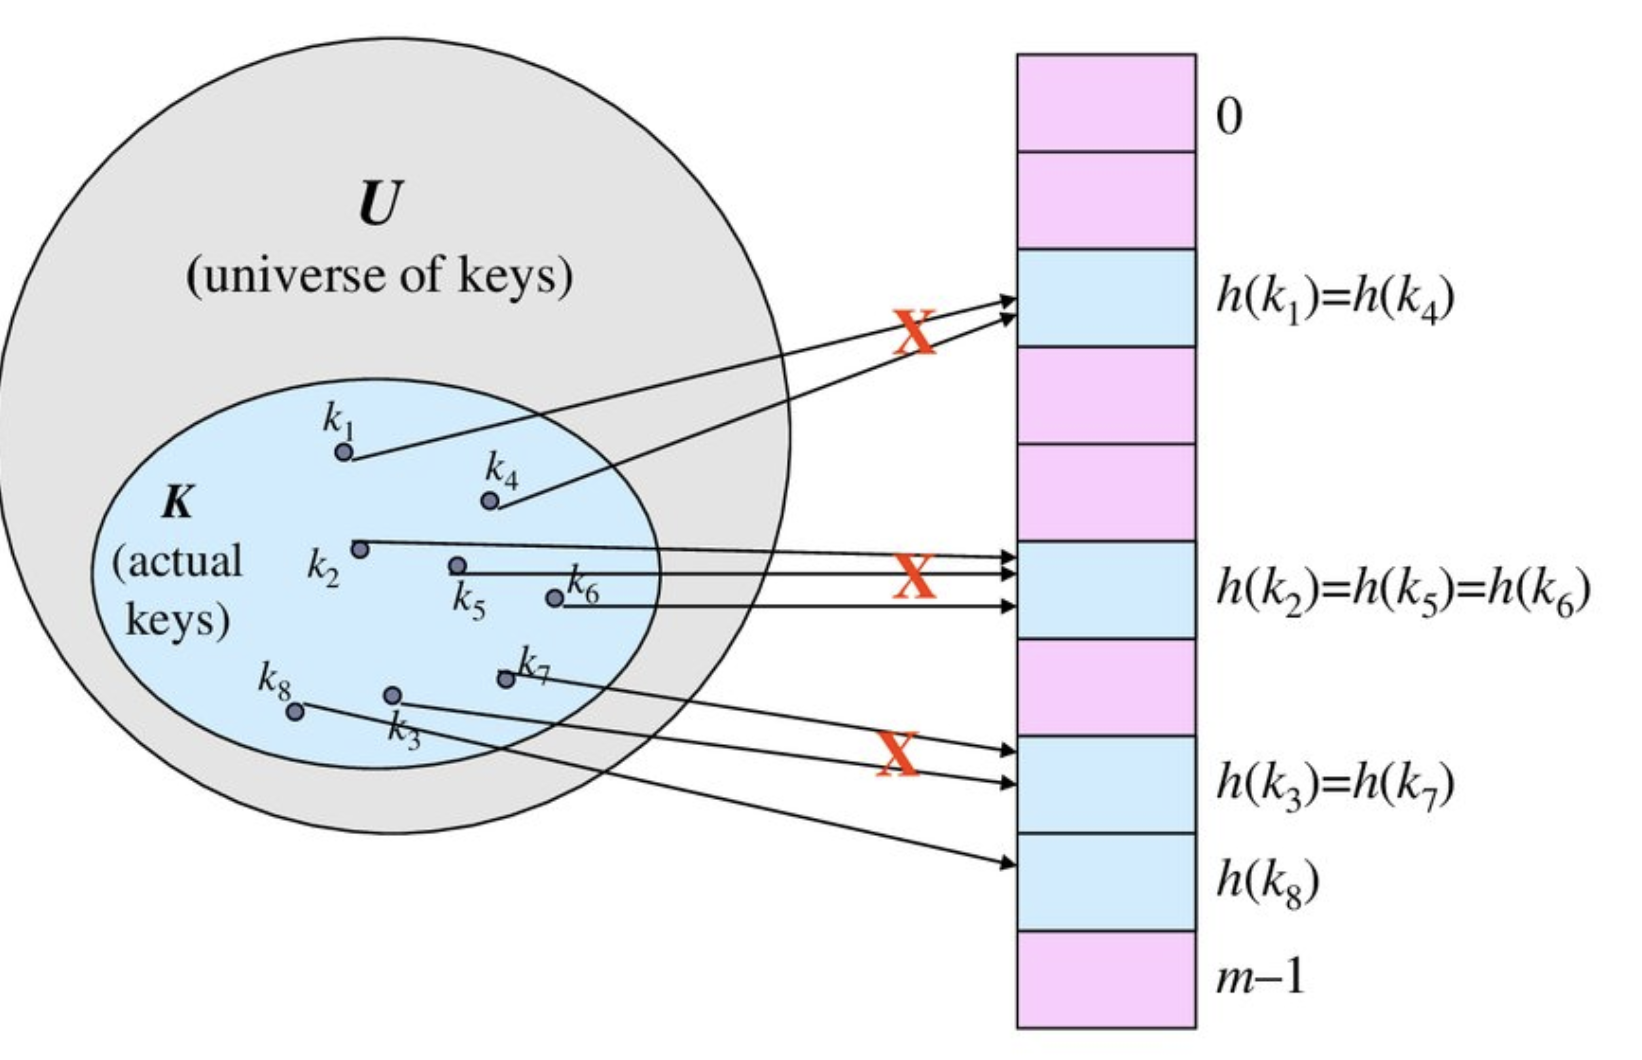
\includegraphics[width=0.8\textwidth]{aulas/aula2-hash-fig2.png}
    \caption{Tratamento de Colisões}
  \end{figure}
\end{frame}

% Slide 2: Métodos de Tratamento de Colisões

\begin{frame}[fragile]
  \frametitle{Métodos de Tratamento de Colisões}
  \begin{itemize}
    \item Encadeamento externo:
      \begin{itemize}
        \item No método de encadeamento externo, cada entrada da tabela de dispersão mantém uma lista encadeada de todos os elementos que colidem naquele índice específico.
        \item Quando ocorre uma colisão, o novo elemento é simplesmente adicionado à lista encadeada correspondente.
        \item Este método é simples de implementar e eficaz para lidar com colisões, especialmente em cenários onde as colisões são frequentes.
        \item No entanto, pode exigir mais espaço de memória devido à necessidade de armazenar as listas encadeadas.
      \end{itemize}
  \end{itemize}
\end{frame}

\begin{frame}[fragile]
  \frametitle{Tratamento de Colisões - Encadeamento}
  \begin{figure}
    \centering
    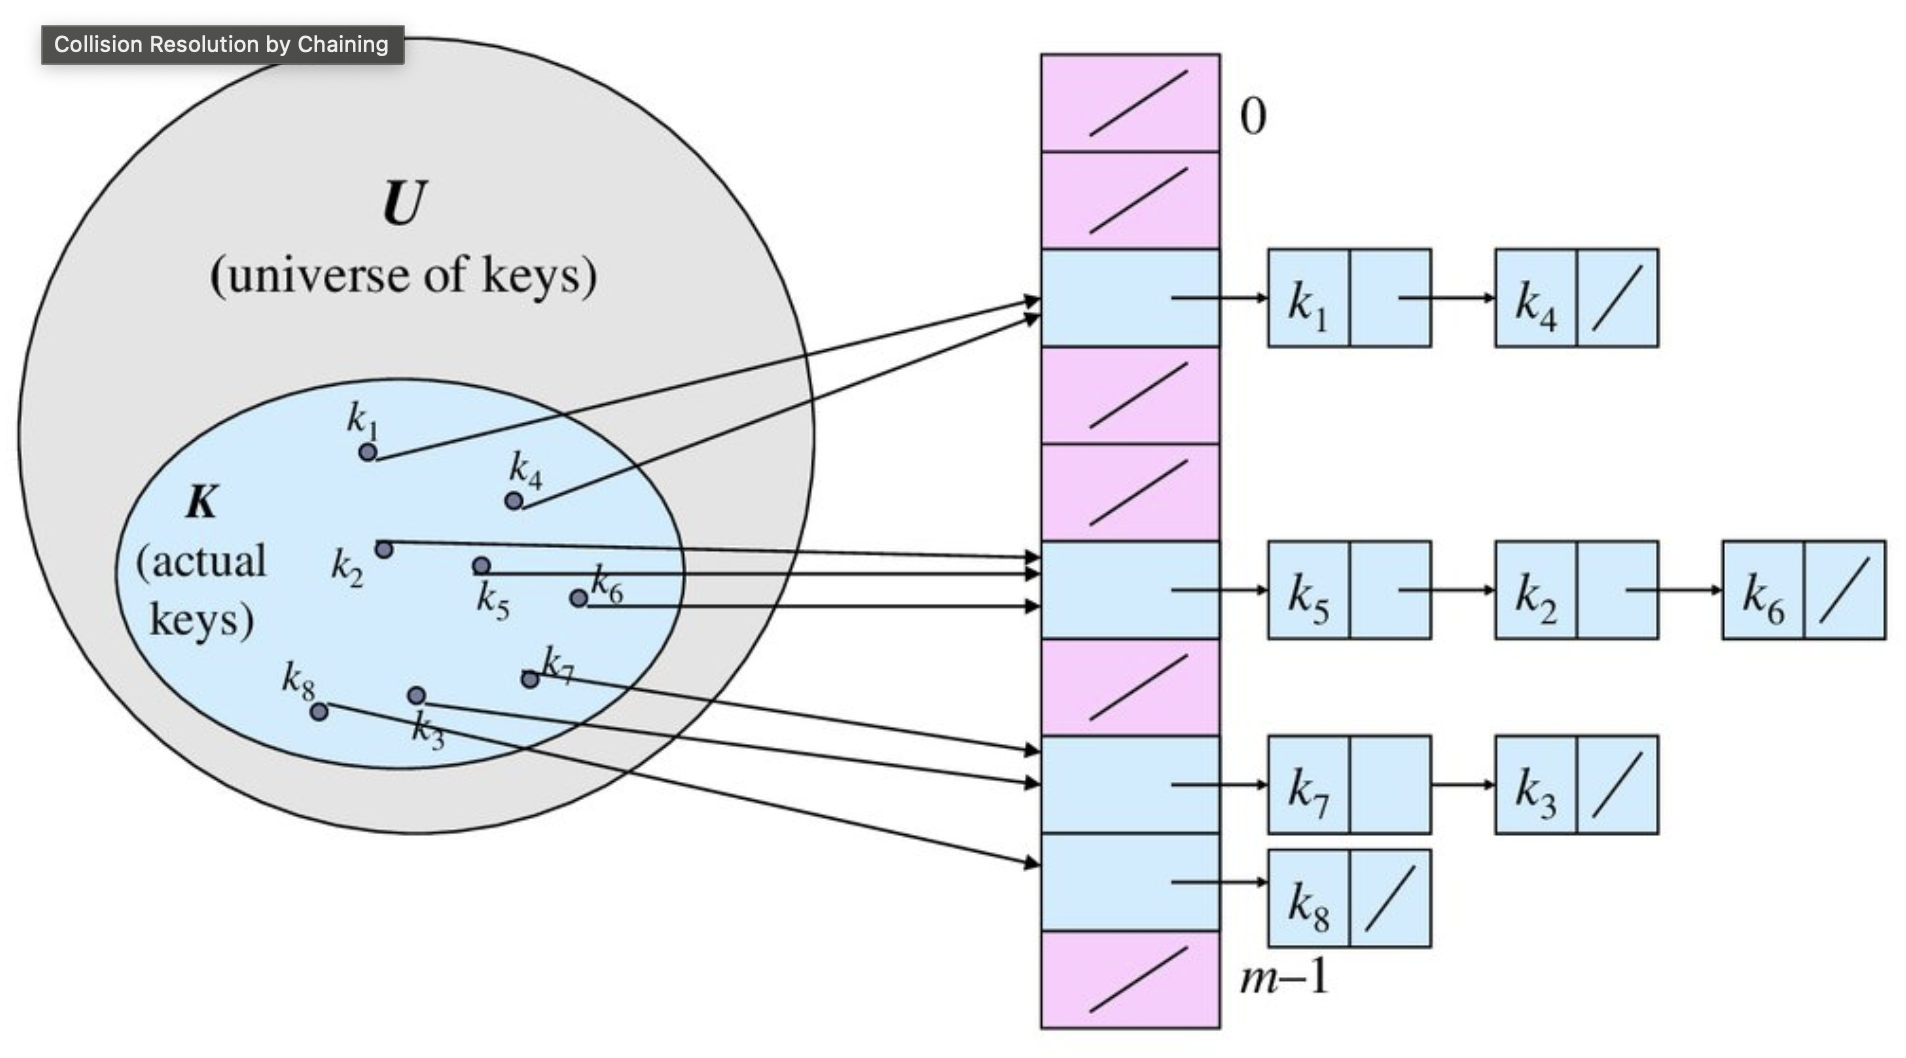
\includegraphics[width=0.8\textwidth]{aulas/aula2-hash-fig3.png}
    \caption{Tratamento de Colisões}
  \end{figure}
\end{frame}


\begin{frame}[fragile]
  \frametitle{Métodos de Tratamento de Colisões}
  \begin{itemize}
    \item Endereçamento aberto:
      \begin{itemize}
        \item O endereçamento aberto é uma abordagem em que, quando ocorre uma colisão, a tabela de dispersão é pesquisada por outra posição livre para inserir o novo elemento.
        \item Existem várias técnicas de endereçamento aberto, incluindo sondagem linear, sondagem quadrática e hashing duplo.
        \item Estas técnicas diferem na forma como procuram por posições alternativas na tabela quando ocorre uma colisão.
        \item O endereçamento aberto pode ser mais eficiente em termos de uso de memória, mas requer cuidados especiais para evitar clusters de colisões.
      \end{itemize}
  \end{itemize}
\end{frame}


% Slide 3: Exemplos e Análise de Métodos de Tratamento de Colisões

\begin{frame}[fragile]
  \frametitle{Exemplos e Análise de Métodos de Tratamento de Colisões}
Comparação dos métodos de tratamento de colisões:
      \begin{itemize}
        \item Encadeamento externo:
          \begin{itemize}
            \item No método de encadeamento externo, as colisões são tratadas armazenando múltiplos elementos que colidem no mesmo índice em uma estrutura de dados separada, como uma lista encadeada.
            \item Vantagens:
              \begin{itemize}
                \item Fácil implementação.
                \item Eficiente para lidar com colisões frequentes.
              \end{itemize}
            \item Desvantagens:
              \begin{itemize}
                \item Pode consumir mais espaço de memória devido à necessidade de armazenar listas encadeadas.
                \item Pode levar a acessos indiretos adicionais durante a busca de elementos.
              \end{itemize}
          \end{itemize}
      \end{itemize}
\end{frame}

\begin{frame}[fragile]
  \frametitle{Exemplos e Análise de Métodos de Tratamento de Colisões (Continuação)}
Comparação dos métodos de tratamento de colisões (cont.):
      \begin{itemize}
        \item Endereçamento aberto:
          \begin{itemize}
            \item No endereçamento aberto, quando ocorre uma colisão, novas posições na tabela de dispersão são pesquisadas para encontrar um local alternativo para o novo elemento.
            \item Vantagens:
              \begin{itemize}
                \item Mais eficiente em termos de uso de memória, pois não requer estruturas de dados adicionais.
                \item Pode ser mais rápido em alguns cenários, especialmente quando as colisões são raras.
              \end{itemize}
            \item Desvantagens:
              \begin{itemize}
                \item Requer técnicas adicionais para lidar com clusters de colisões.
                \item Pode ser mais complicado de implementar.
              \end{itemize}
          \end{itemize}
      \end{itemize}
\end{frame}

\begin{frame}[fragile]
  \frametitle{Exemplos e Análise de Métodos de Tratamento de Colisões (Continuação)}
  Discussão sobre as vantagens e desvantagens de cada método:
  \begin{itemize}
    \item A escolha entre encadeamento externo e endereçamento aberto 
    depende das características específicas do problema, como a 
    distribuição das chaves e a frequência de colisões.
  \end{itemize}
\end{frame}

% Slide 4: Prática - Implementando e Testando o Tratamento de Colisões
\begin{frame}[fragile]
  \frametitle{Prática - Implementando e Testando o Tratamento de Colisões (Parte 1)}
  \begin{verbatim}
    // Exemplo de encadeamento externo em pseudocódigo
    inserir(chave, valor):
      indice = funcao_hash(chave)
      se tabela[indice] não está vazia:
        inserir na lista encadeada
      senão:
        criar nova entrada
  \end{verbatim}
  \begin{itemize}
    \item Atividade prática: Implementação e testes com diferentes cenários de colisões.
  \end{itemize}
\end{frame}

\begin{frame}[fragile]
  \frametitle{Prática - Implementando e Testando o Tratamento de Colisões (Parte 2)}
  \textbf{Exemplo de Encadeamento Externo:}
  \begin{itemize}
    \item Suponha que temos uma tabela de dispersão de tamanho 5 e a seguinte sequência de chaves é inserida: 7, 12, 3, 8, 18.
    \item A função hash poderia ser algo como "chave \% 5".
    \item Quando ocorre uma colisão, inserimos na lista encadeada correspondente.
  \end{itemize}
\end{frame}
\begin{frame}[fragile]
  \frametitle{Prática - Implementando e Testando o Tratamento de Colisões (Parte 3)}
  \textbf{Exemplo de Endereçamento Aberto:}
  \begin{itemize}
    \item Suponha a mesma tabela de dispersão de tamanho 5 e a mesma sequência de chaves é inserida.
    \item A função hash poderia ser "chave \% 5".
    \item Quando ocorre uma colisão, procuramos por uma posição alternativa na tabela para inserir a chave.
  \end{itemize}
\end{frame}

\begin{frame}[fragile]{Descrição do Problema: Dois Soma}
O problema "Dois Soma" (Two Sum) é um desafio de codificação clássico 
usado em entrevistas de emprego e prática de algoritmos. O objetivo é 
encontrar dois números em um array de inteiros que somem um valor alvo 
específico.

Requisitos:
\begin{itemize}
  \item Dado um array de inteiros `numeros` e um inteiro `alvo`.
  \item Retornar os índices dos dois números de tal forma que eles somem ao `alvo`.
  \item Você pode assumir que cada entrada teria exatamente uma solução, e você não pode usar o mesmo elemento duas vezes.
  \item A resposta pode ser retornada em qualquer ordem.
\end{itemize}

\end{frame}
\begin{frame}{Descrição das Entradas e Saídas}
  \textbf{Entradas:}
  \begin{itemize}
      \item Um \textit{array} de inteiros \texttt{numeros}.
      \item Um inteiro \texttt{alvo}, representando o valor alvo a ser alcançado pela soma de dois números no array.
  \end{itemize}
  
  \textbf{Saídas:}
  \begin{itemize}
      \item Uma lista contendo os índices dos \textit{dois números} dentro do array \texttt{numeros} que somam para o valor \texttt{alvo}.
  \end{itemize}
  
  \textbf{Exemplo:}
  \begin{itemize}
      \item \textbf{Entrada:} \texttt{numeros = [2, 7, 11, 15]}, \texttt{alvo = 9}
      \item \textbf{Saída:} \texttt{[0, 1]}
      \item \textbf{Explicação:} \texttt{numeros[0] + numeros[1] == 9}, portanto, retornamos \texttt{[0, 1]}.
  \end{itemize}
\end{frame}
\begin{frame}{Casos de Teste}
  \begin{block}{Caso de Teste 1}
      \textbf{Entrada:} \texttt{numeros = [2, 7, 11, 15]}, \texttt{alvo = 9}\\
      \textbf{Saída esperada:} \texttt{[0, 1]}
  \end{block}

  \begin{block}{Caso de Teste 2}
      \textbf{Entrada:} \texttt{numeros = [3, 2, 4]}, \texttt{alvo = 6}\\
      \textbf{Saída esperada:} \texttt{[1, 2]}
  \end{block}

  \begin{block}{Caso de Teste 3}
      \textbf{Entrada:} \texttt{numeros = [3, 3]}, \texttt{alvo = 6}\\
      \textbf{Saída esperada:} \texttt{[0, 1]}
  \end{block}

  \begin{block}{Caso de Teste 4}
      \textbf{Entrada:} \texttt{numeros = [-1, -2, -3, -4, -5]}, \texttt{alvo = -8}\\
      \textbf{Saída esperada:} \texttt{[2, 4]}
  \end{block}
\end{frame}
\begin{frame}[fragile]{Solução do problema "Dois Soma" em JavaScript}
  \small
  \begin{lstlisting}
  function doisSoma(numeros, alvo) {
      // Inicializa um objeto para mapear os numeros aos seus indices
      let mapa = {}; 
      for (let i = 0; i < numeros.length; i++) {
        // Calcula o complemento do numero atual
          const complemento = alvo - numeros[i]; 
          // Verifica se o complemento já existe no mapa
          if (mapa[complemento] !== undefined) {
            // Retorna os indices do complemento e do numero atual    
          return [mapa[complemento], i]; 
          }
          // Adiciona o numero atual ao mapa com seu indice
          mapa[numeros[i]] = i; 
      }
      // Retorna uma lista vazia se nenhum par for encontrado
      return []; 
  }
  \end{lstlisting}
\end{frame}

\begin{frame}[fragile]{Contexto do Problema}
  Imagine o restaurante "Sabor e Arte", famoso pela sua cozinha inovadora e diversificada. A cada mês, o restaurante introduz novos pratos ao menu, buscando surpreender e satisfazer seus clientes. Para entender melhor quais pratos são os mais apreciados, o restaurante coleta avaliações dos clientes, que vão de 0 a 5 estrelas.
  
  Com o aumento do número de avaliações, tornou-se desafiador para a equipe do restaurante identificar rapidamente quais pratos estão fazendo mais sucesso. Eles precisam de uma solução que calcule automaticamente a média das avaliações de cada prato e destaque o prato com a melhor média. Em caso de empate nas médias, o prato introduzido mais recentemente (assumindo que tem o ID mais alto) deve ser considerado o menos favorito, como forma de incentivar a inovação constante.
  
  O desafio é desenvolver um algoritmo que ajude o "Sabor e Arte" a reconhecer o prato estrela de cada mês, otimizando sua oferta e garantindo a satisfação dos clientes.
\end{frame}
    

  \begin{frame}[fragile]{Descrição do Problema e Restrições}
    \begin{itemize}
        \item Dado um array de pares, onde cada par consiste em um identificador de produto (\texttt{id}) e uma avaliação dada por um cliente (\texttt{rating}).
        \item Os \texttt{id} dos produtos variam de 1 a 5000.
        \item As avaliações (\texttt{rating}) variam de 0 a 5.
        \item O objetivo é calcular a média das avaliações de cada produto.
        \item Deve-se retornar o produto com a maior avaliação média.
        \item Se dois produtos possuírem a mesma média, retorna o produto com o ID menor.
    \end{itemize}
\end{frame}

\begin{frame}[fragile]{Casos de Teste Adicionais}
  \textbf{Caso de Teste 4:} 8 elementos\
  Entrada: \texttt{[[4001, 3], [4002, 2], [4001, 4], [4003, 5], [4001, 5], [4004, 1], [4005, 4], [4001, 3]]}\
  Saída esperada: \texttt{4001}
  
  \textbf{Caso de Teste 5:} 6 elementos\
  Entrada: \texttt{[[5001, 5], [5002, 5], [5003, 3], [5004, 3], [5002, 4], [5001, 4]]}\
  Saída esperada: \texttt{5001} \textit{(5001 tem id menor que 5002)}
  
  \textbf{Caso de Teste 6:} 4 elementos\
  Entrada: \texttt{[[6001, 1], [6002, 2], [6003, 3], [6004, 4]]}\
  Saída esperada: \texttt{6004}
  \end{frame}

\begin{frame}[fragile]{Solução em JavaScript}
  \begin{lstlisting}[language=JavaScript]
  function encontrarMelhorAvaliacao(avaliacoes) {
      const somaAvaliacoes = {};
      const contagemAvaliacoes = {};
      avaliacoes.forEach(([id, rating]) => {
          if (somaAvaliacoes[id]) {
              somaAvaliacoes[id] += rating;
              contagemAvaliacoes[id] += 1;
          } else {
              somaAvaliacoes[id] = rating;
              contagemAvaliacoes[id] = 1;
          }
      });
      ...
  }
  \end{lstlisting}
\end{frame}
\begin{frame}[fragile]{Solução em JavaScript}
  \begin{lstlisting}[language=JavaScript]
  function encontrarMelhorAvaliacao(avaliacoes) {
      ...
      let melhorId = null;
      let maiorMedia = 0;
      for (const id in somaAvaliacoes) {
          const media = somaAvaliacoes[id] / contagemAvaliacoes[id];
          if (media > maiorMedia || (media === maiorMedia && (melhorId === null || parseInt(id) < melhorId))) {
              maiorMedia = media;
              melhorId = id;
          }
      }
      return melhorId;
  }
  \end{lstlisting}
  \end{frame}
  
